\documentclass[10pt,letterpaper]{article}
\usepackage[top=0.85in,left=2.75in,footskip=0.75in]{geometry}
\usepackage{bibentry}

% Text layout specific to Supplemental Materials
\topmargin 0.0cm
\oddsidemargin 0.5cm
\evensidemargin 0.5cm
\textwidth 16cm
\textheight 21cm

\setlength{\parskip}{1em}

% Template for PLoS
% Version 3.2 March 2016

% General commands for text/figures

% Page margin
\usepackage[top=0.85in,left=2.75in,footskip=0.75in]{geometry}
% Use Unicode characters when possible
\usepackage[utf8x]{inputenc}
% amsmath package, useful for mathematical formulas
\usepackage{amsmath}
%\usepackage{natbib}
% amssymb package, useful for mathematical symbols
\usepackage{amssymb}
%\usepackage{booktabs}
\usepackage{xspace}
\usepackage{hyperref}
% graphicx package, useful for including eps and pdf graphics
% include graphics with the command \includegraphics
\usepackage{graphicx}

% Use adjustwidth environment to exceed column width (see example table in text)
\usepackage{changepage}

% textcomp package and marvosym package for additional characters
\usepackage{textcomp,marvosym}

% fixltx2e package for \textsubscript
\usepackage{fixltx2e}

% cite package, to clean up citations in the main text. Do not remove.
\usepackage{cite}
\usepackage{caption}
\usepackage{subcaption}
\usepackage{rotating}

\usepackage{color}

% Use doublespacing - comment out for single spacing
%\usepackage{setspace}
%\doublespacing


% Bold the 'Figure #' in the caption and separate it with a period
% Captions will be left justified
\usepackage[labelfont=bf,labelsep=period,justification=raggedright]{caption}

% Use the PLoS provided bibtex style
%\bibliographystyle{/Users/stephens/Dropbox/Documents/stylefiles/plos2009}

% Remove brackets from numbering in List of References
\makeatletter
\renewcommand{\@biblabel}[1]{\quad#1.}
\makeatother

% Use nameref to cite supporting information files (see Supporting Information section for more info)
\usepackage{nameref,hyperref}

% line numbers
%\usepackage[right]{lineno}

% ligatures disabled
\usepackage{microtype}
\DisableLigatures[f]{encoding = *, family = * }

% Leave date blank
\date{}

%\pagestyle{myheadings}
%% ** EDIT HERE **
\usepackage{enumerate}
\usepackage{multirow}
\usepackage{url}
\usepackage{xr} %for cross-referencing
%% ** EDIT HERE **
%% PLEASE INCLUDE ALL MACROS BELOW
\newtheorem{algorithm}{Algorithm}
\newtheorem{proposition}{Proposition}
\newtheorem{restateproposition}{Proposition}
\newtheorem{lemma}{Lemma}
\newtheorem{corollary}{Corollary}
\newtheorem{result}{Result}
\newtheorem{note}{Note}
\newtheorem{definition}{Definition}

\def\KL{\text{KL}}

% Text layout
\raggedright
\setlength{\parindent}{0.5cm}
\textwidth 5.25in
\textheight 8.75in

% Bold the 'Figure #' in the caption and separate it from the title/caption with a period
% Captions will be left justified
\usepackage[aboveskip=1pt,labelfont=bf,labelsep=period,justification=raggedright,singlelinecheck=off]{caption}
\renewcommand{\figurename}{Fig}

%------ bibliography
% Use the PLoS provided BiBTeX style
\bibliographystyle{bmc-mathphys}
% Remove brackets from numbering in List of References
\makeatletter
\renewcommand{\@biblabel}[1]{\quad#1.}
\makeatother


%% Author's settings
\def\KL{\text{KL}}

\pagestyle{empty} %%in order to delete the number at the bottom of the page


\begin{document}
\section*{Supplementary Figures}
\newpage

\begin{figure*}[h!]
\centering
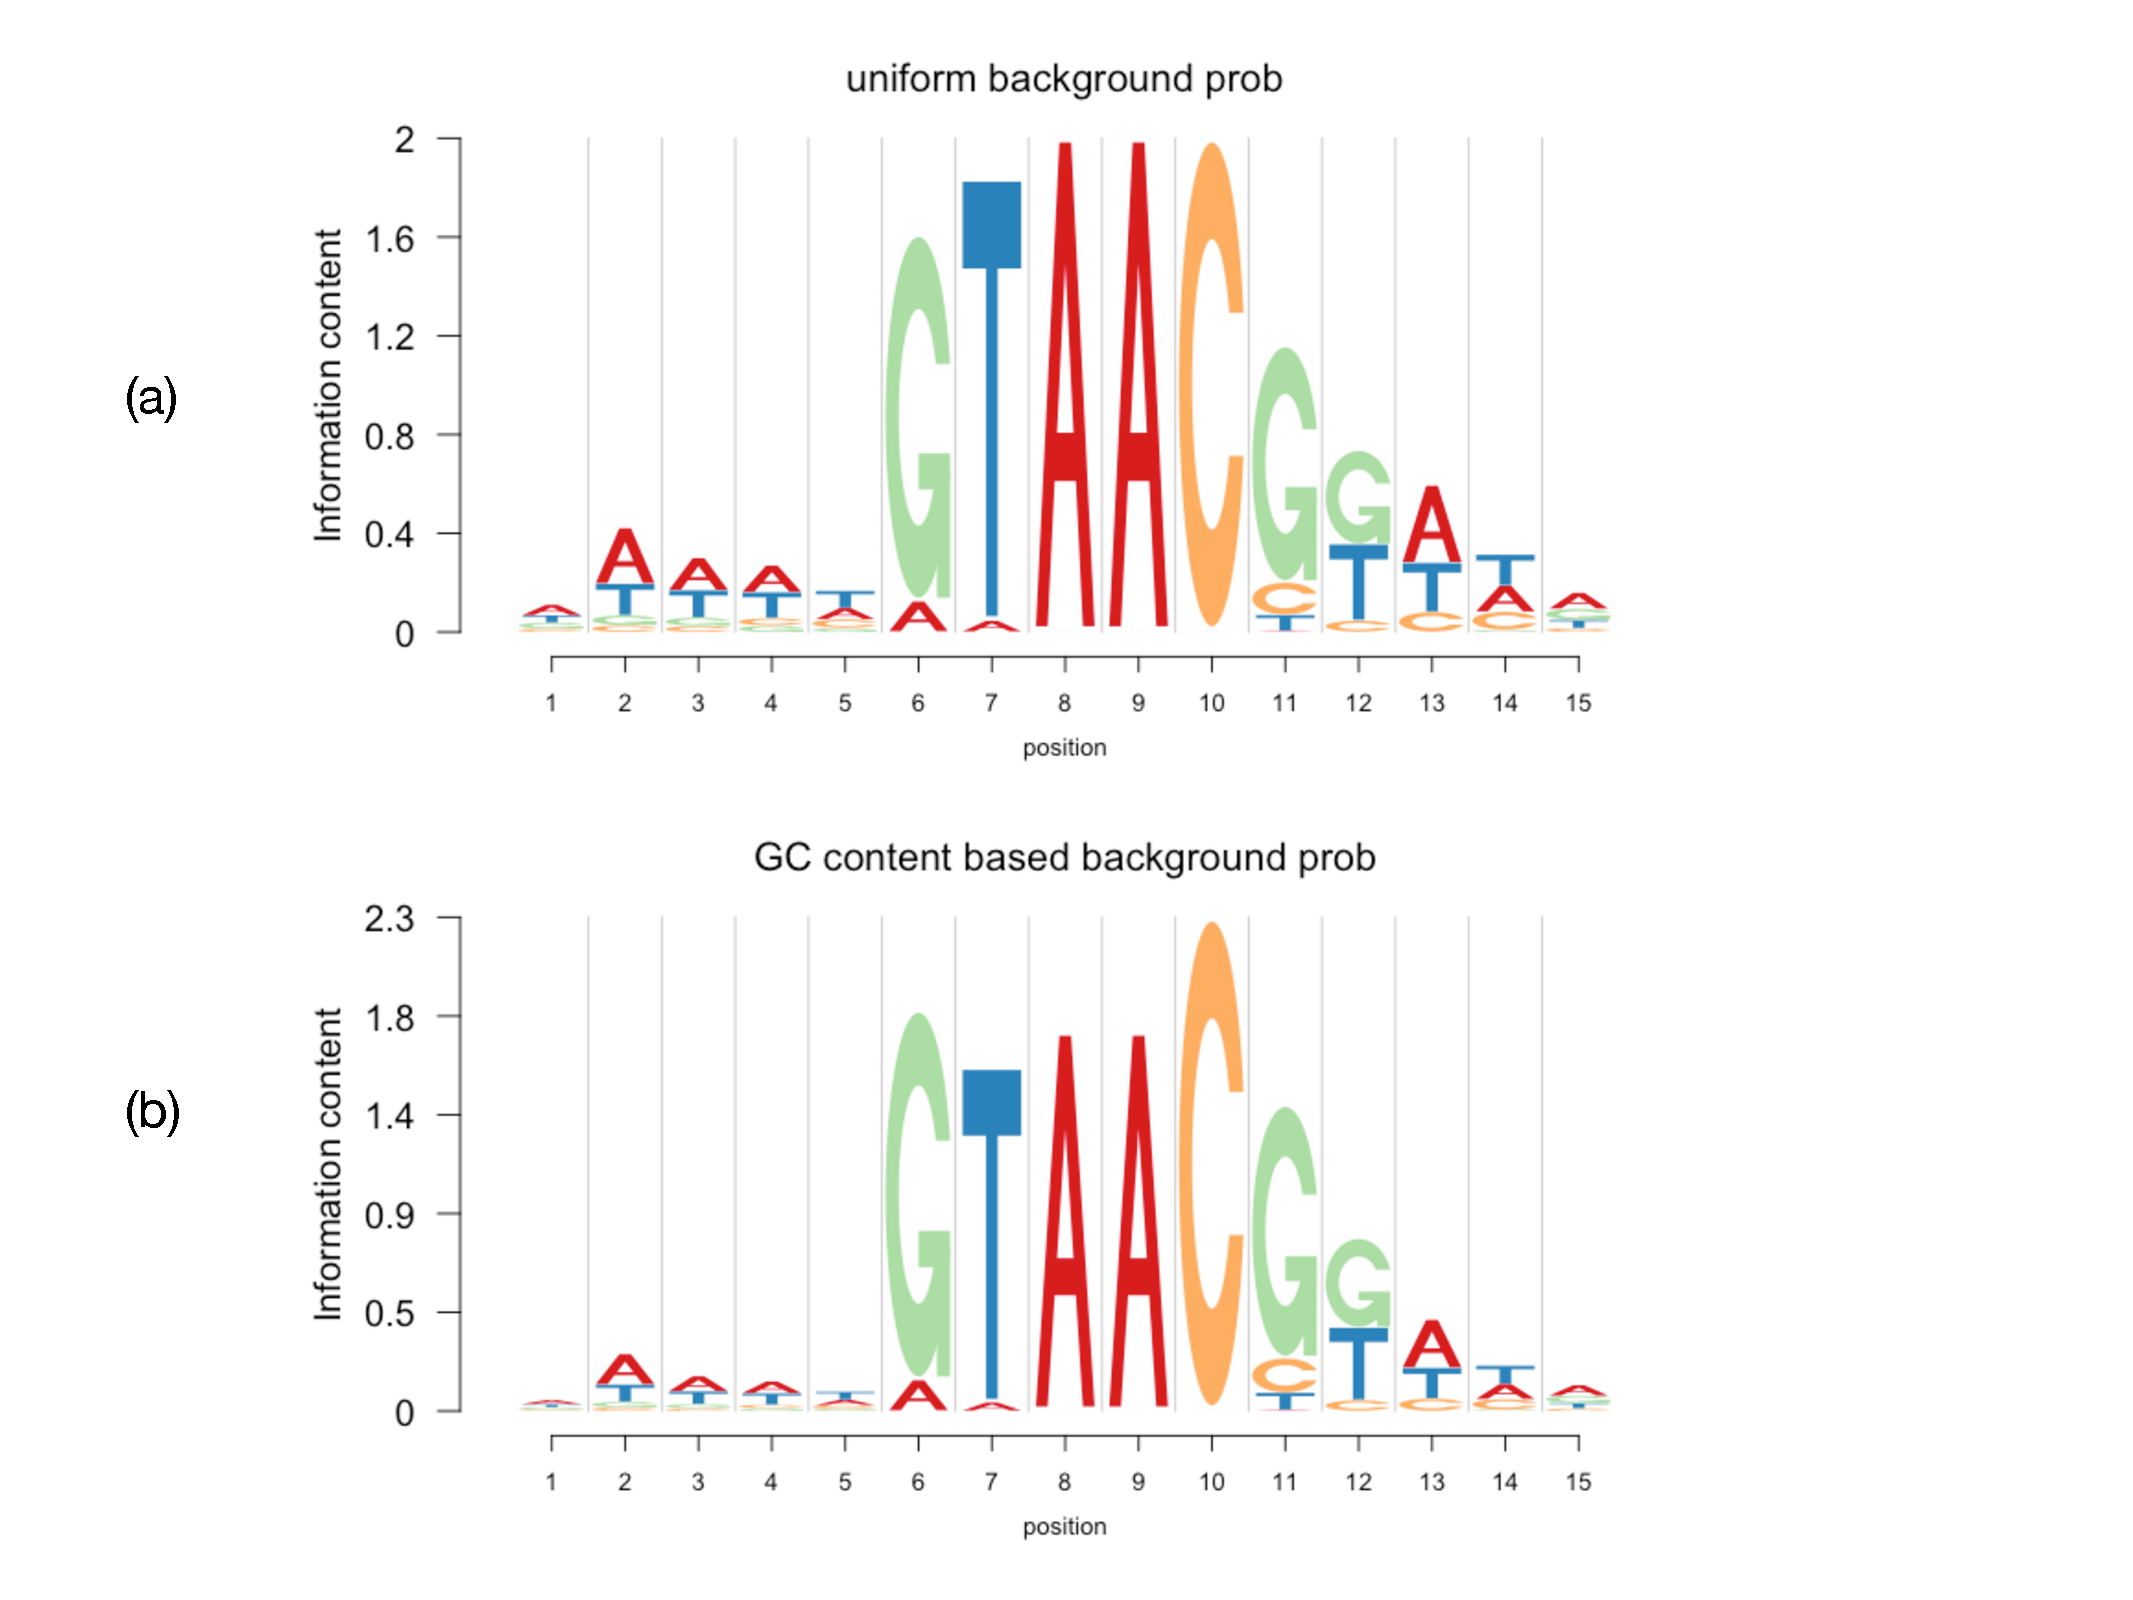
\includegraphics[height=6in, width=7in]{figures_folder/figures1.pdf}
\caption{ \textbf{Standard Logo plot comparison under uniform and non-uniform background base probabilities .}
      Logo plot representation of the plant transcription factor Achn021211 (MYB family protein) in \textit{Actinidia chinensis}. The background probability for this species based on GC content is $q = \left (q_A, q_C, q_G, q_T \right) = \left (0.3141, 0.1859, 0.1859, 0.3141 \right )$. The PWM matrix is obtained from PlantTFDB site (\url{http://planttfdb.cbi.pku.edu.cn/tf.php?sp=Ach&did=Achn021211}). In panel (a), we present the standard logo plot of the PWM matrix with uniform background for all 4 bases. In panel (b), we present the standard logo plot with the above specified background probability.}
\label{fig:suppfig1}
\end{figure*}


\begin{figure*}[h!]
\centering
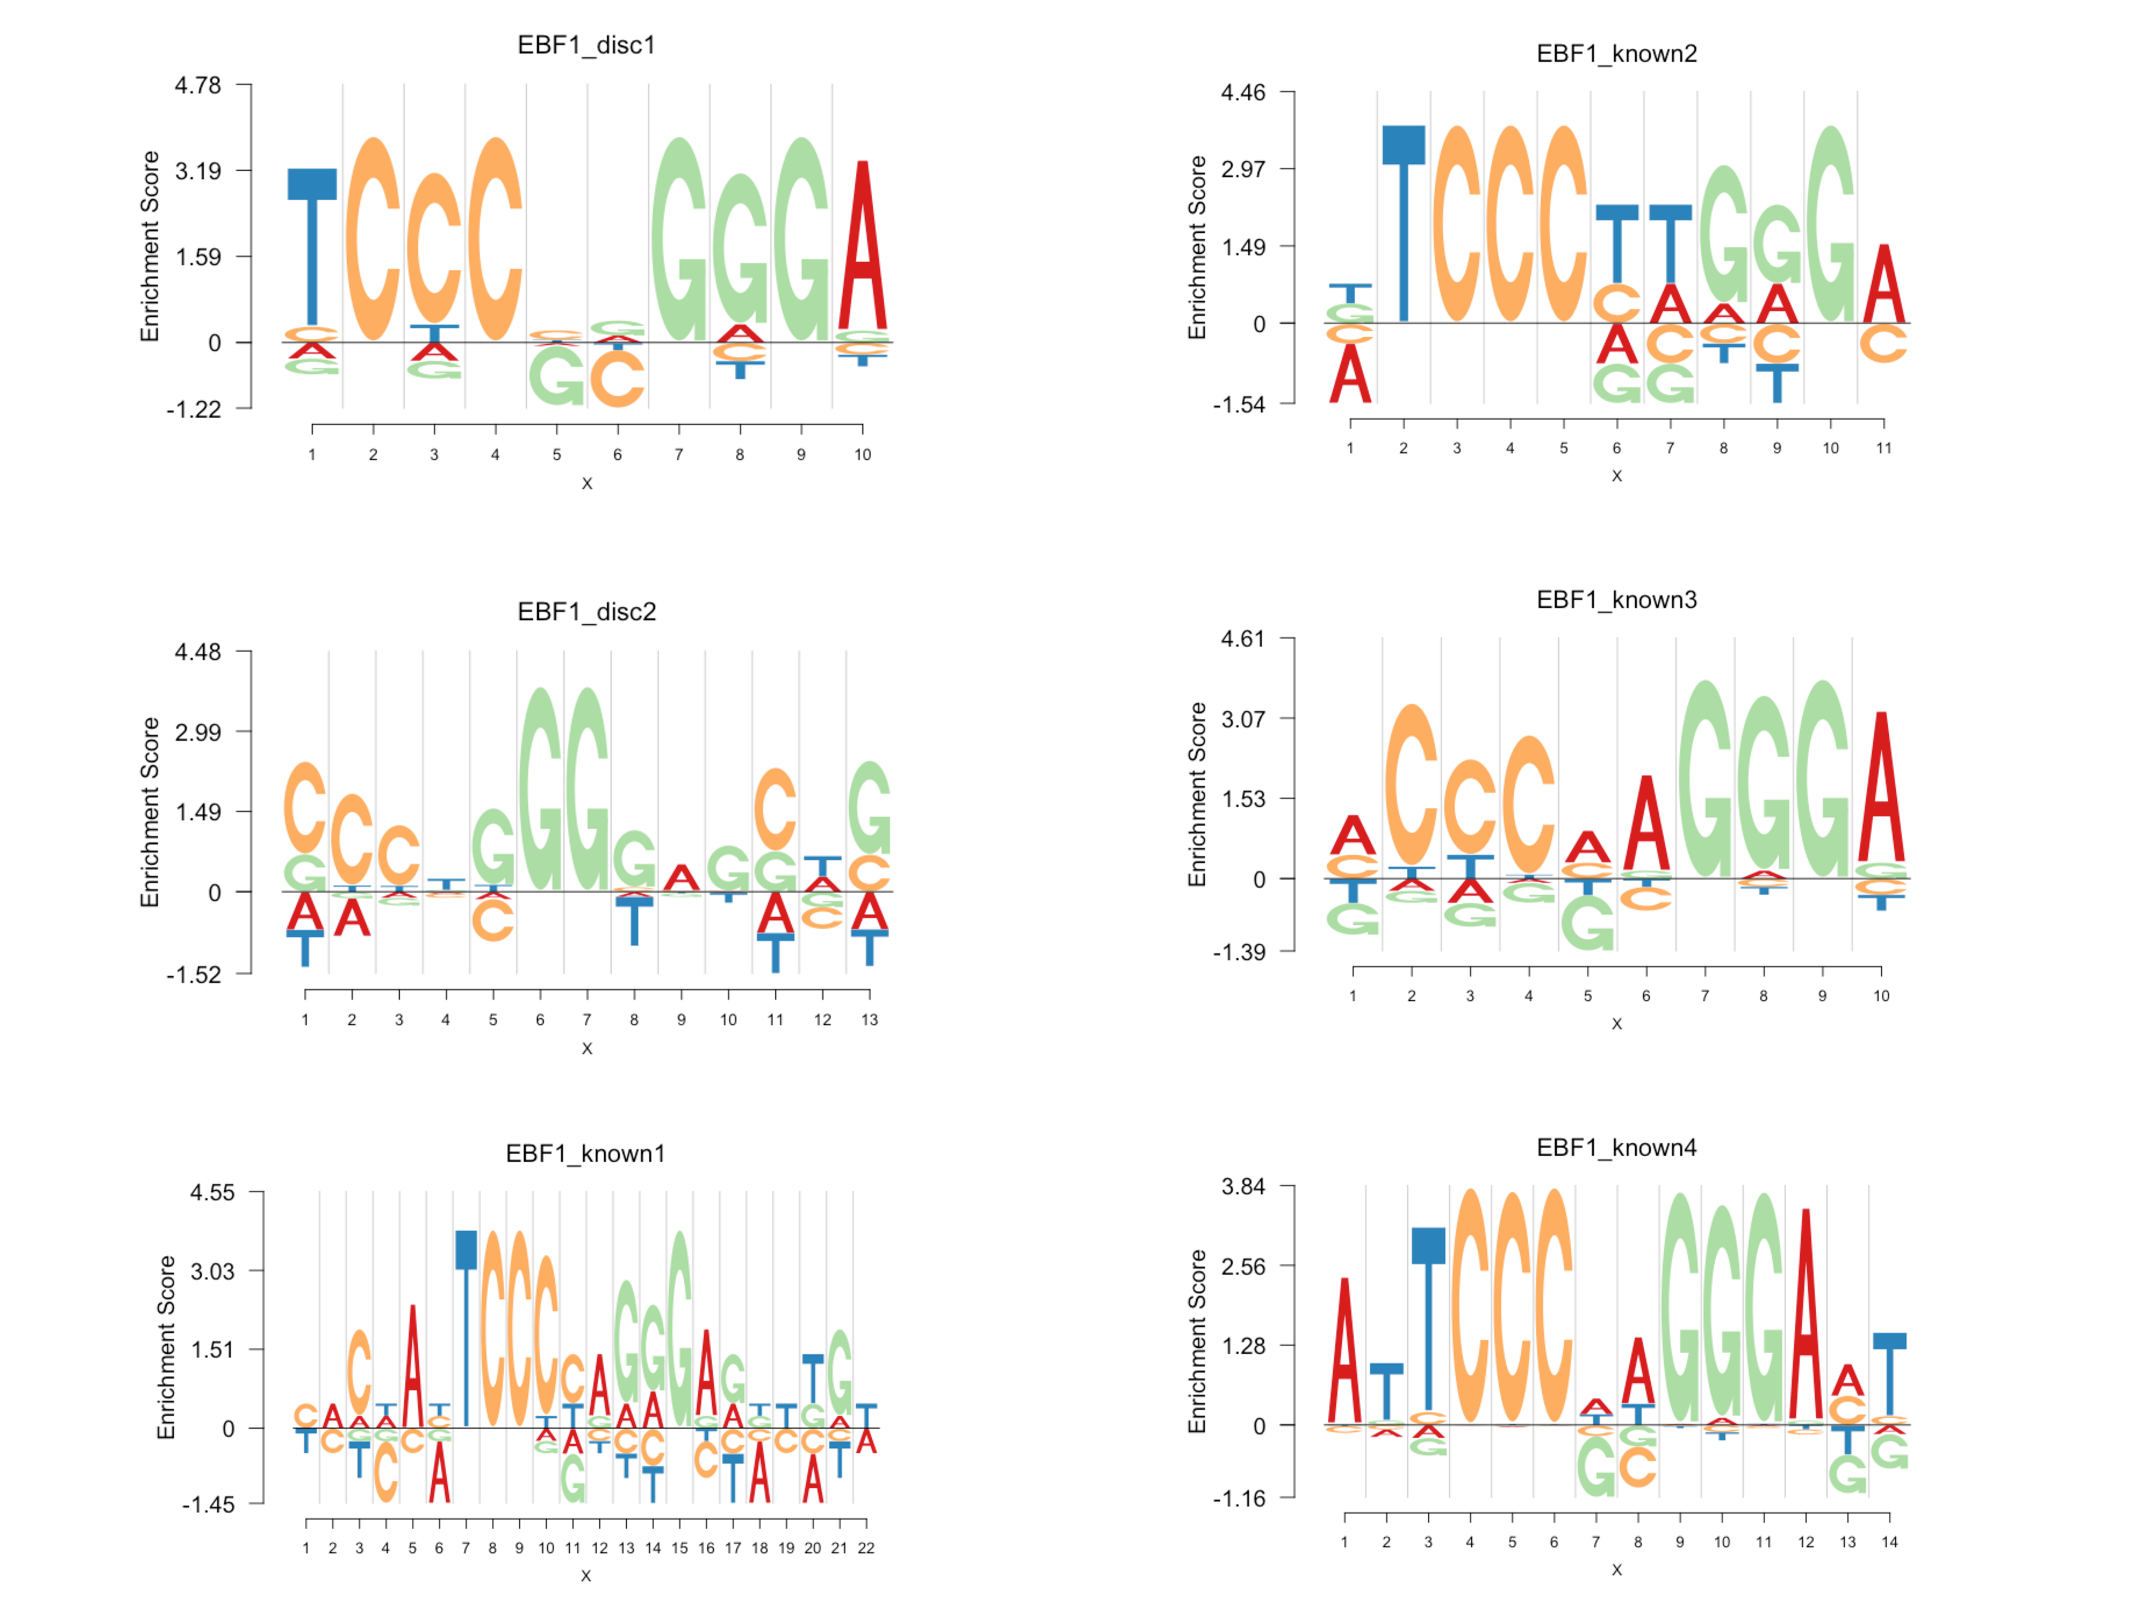
\includegraphics[height=6in, width=7in]{figures_folder/figures6.pdf}
\caption{\textbf{Sparse logo representation of the members of the EBF1 family of transcription factors}: We present the sparse logo representation for the binding sites of 6 transcription factors in the EBF1 family. EBF1-known4 and EBF1-disc1, and also to some extent EBF1-known3 seem to show the depletion of G and C in the middle of the binding site. The PWM data for all the transcription factors have been obtained from the ENCODE TF Chip-seq datasets and are hosted on the webpage \url{http://compbio.mit.edu/encode-motifs/} }
\label{fig:suppfig2}
\end{figure*}

\begin{figure*}[h!]
\centering
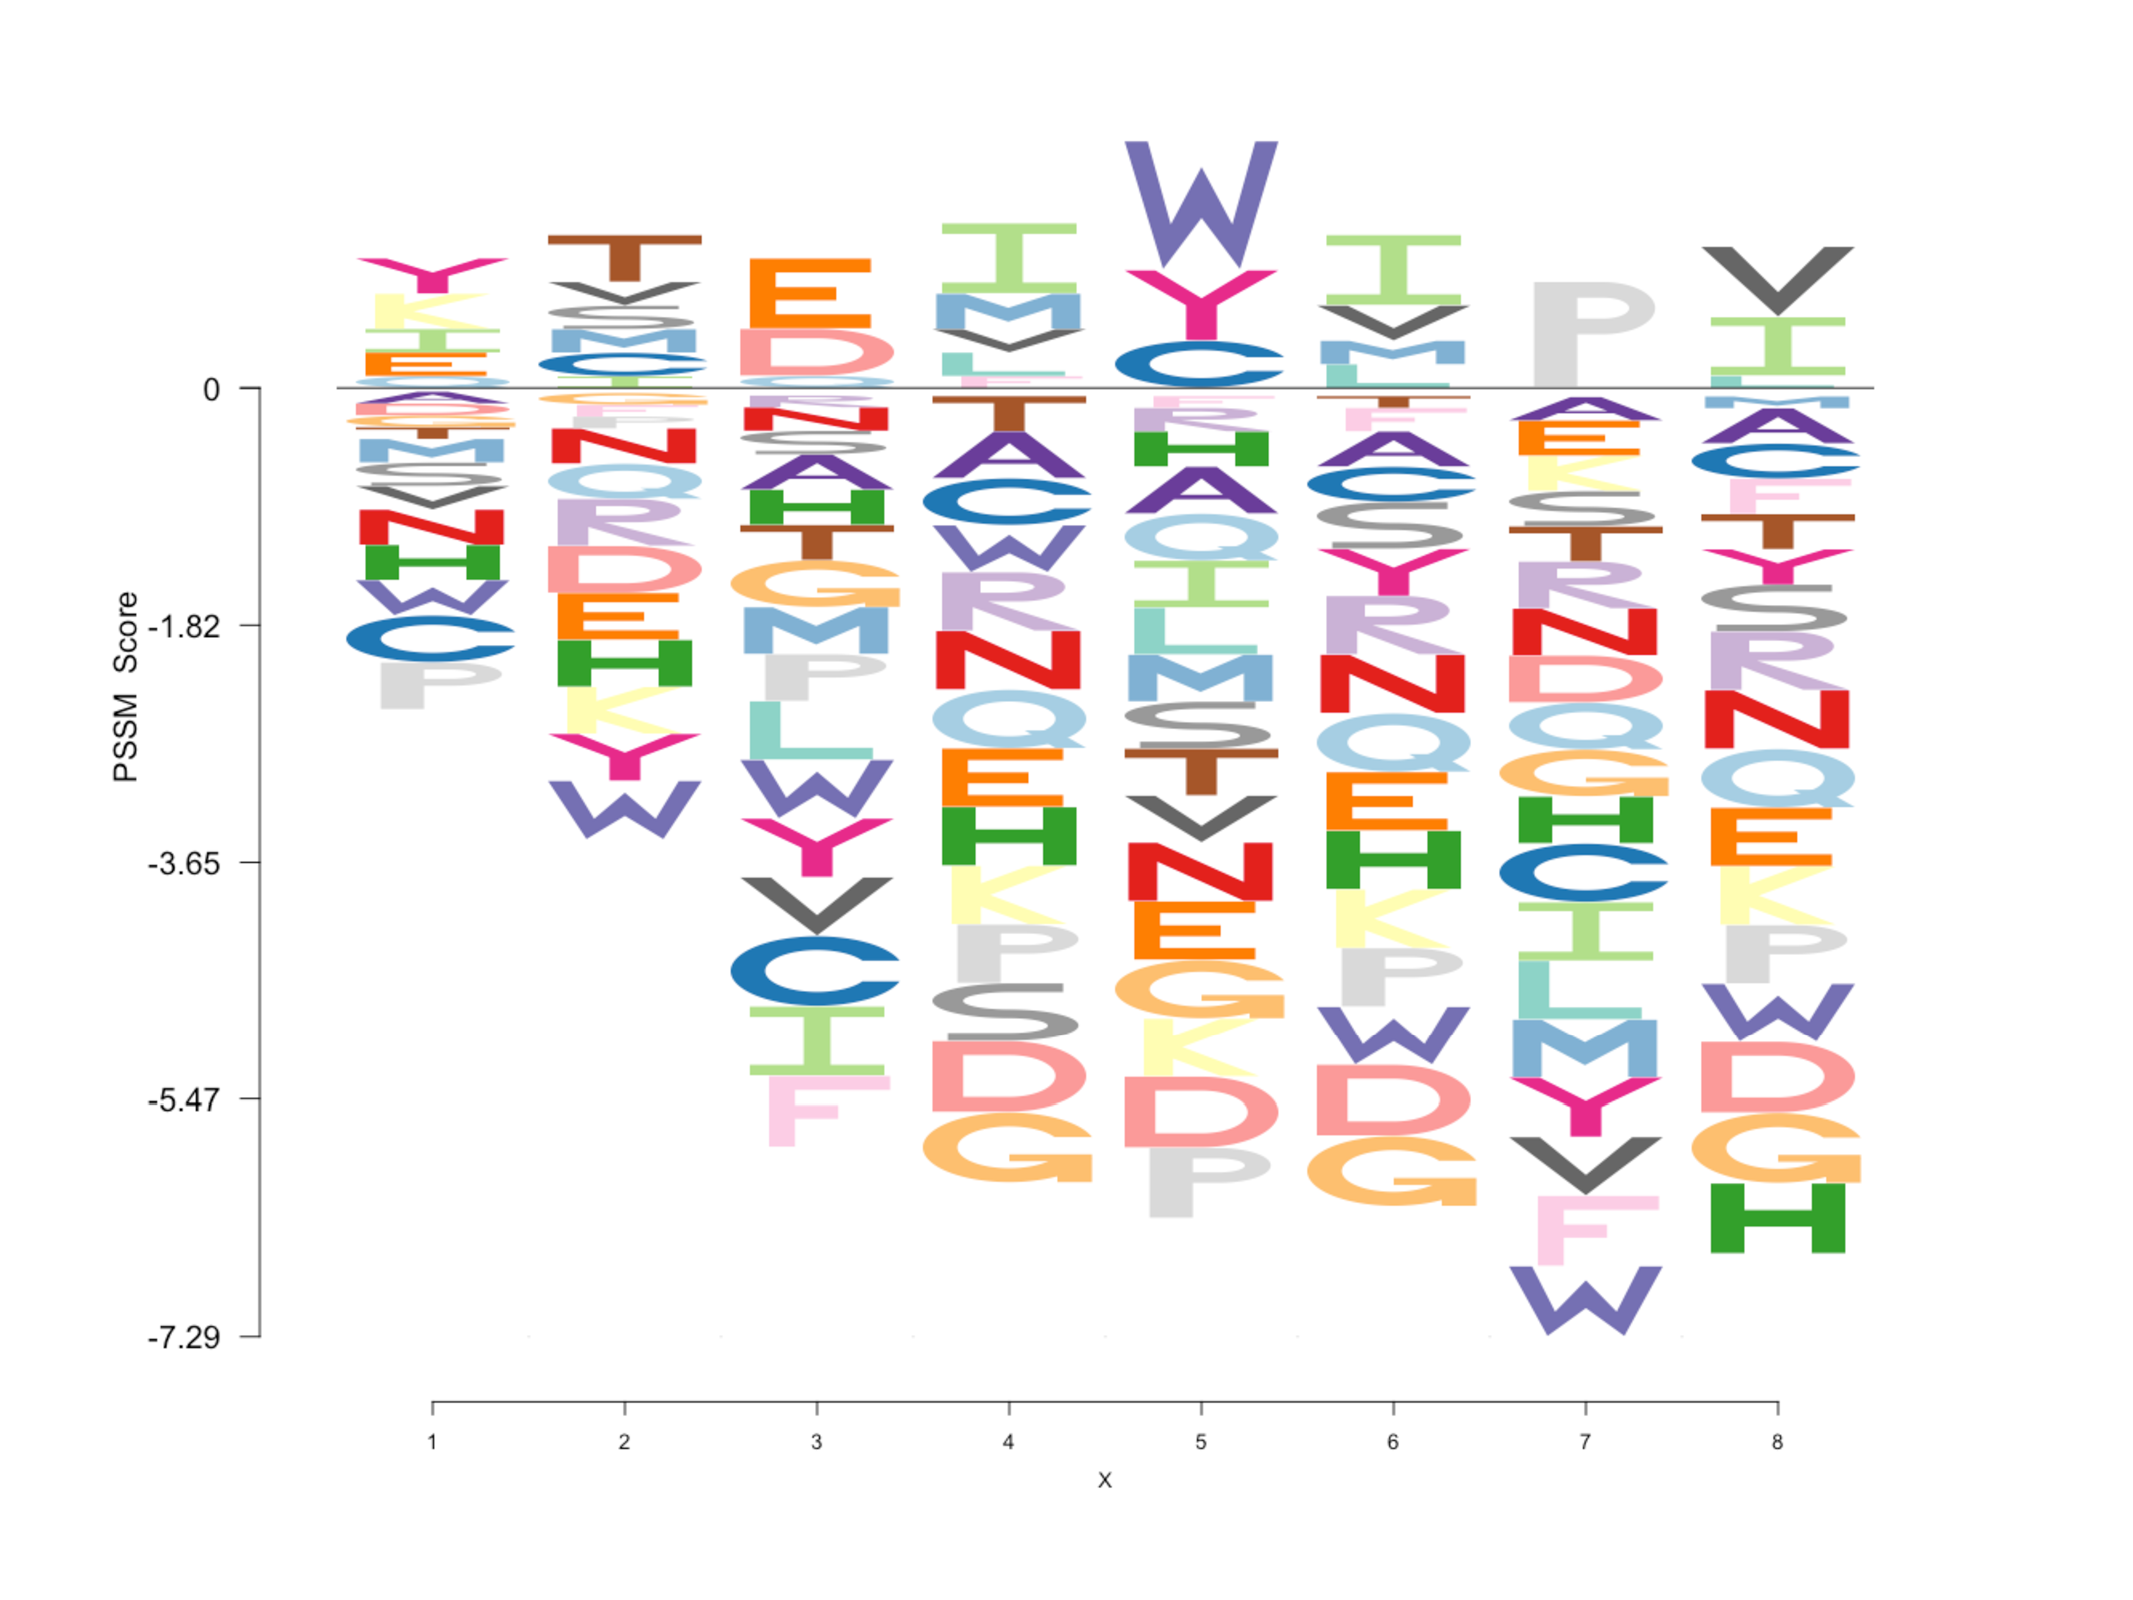
\includegraphics[height=6in, width=7in]{figures_folder/figures14.pdf}
\caption{\textbf{PSSM logo plot for protein sequence motif}: The logo representation of the position specific scoring matrix (PSSM) for the Bacterial transcription activator, effector binding domain protein PF06445 (motif 4, Start=153 Length=8). The data is fetched from the 3PFDB website \url{http://caps.ncbs.res.in/cgi-bin/mini/databases/3pfdb/get_entry.cgi?id=PF06445}}
\label{fig:suppfig3}
\end{figure*}

\begin{figure*}[h!]
\centering
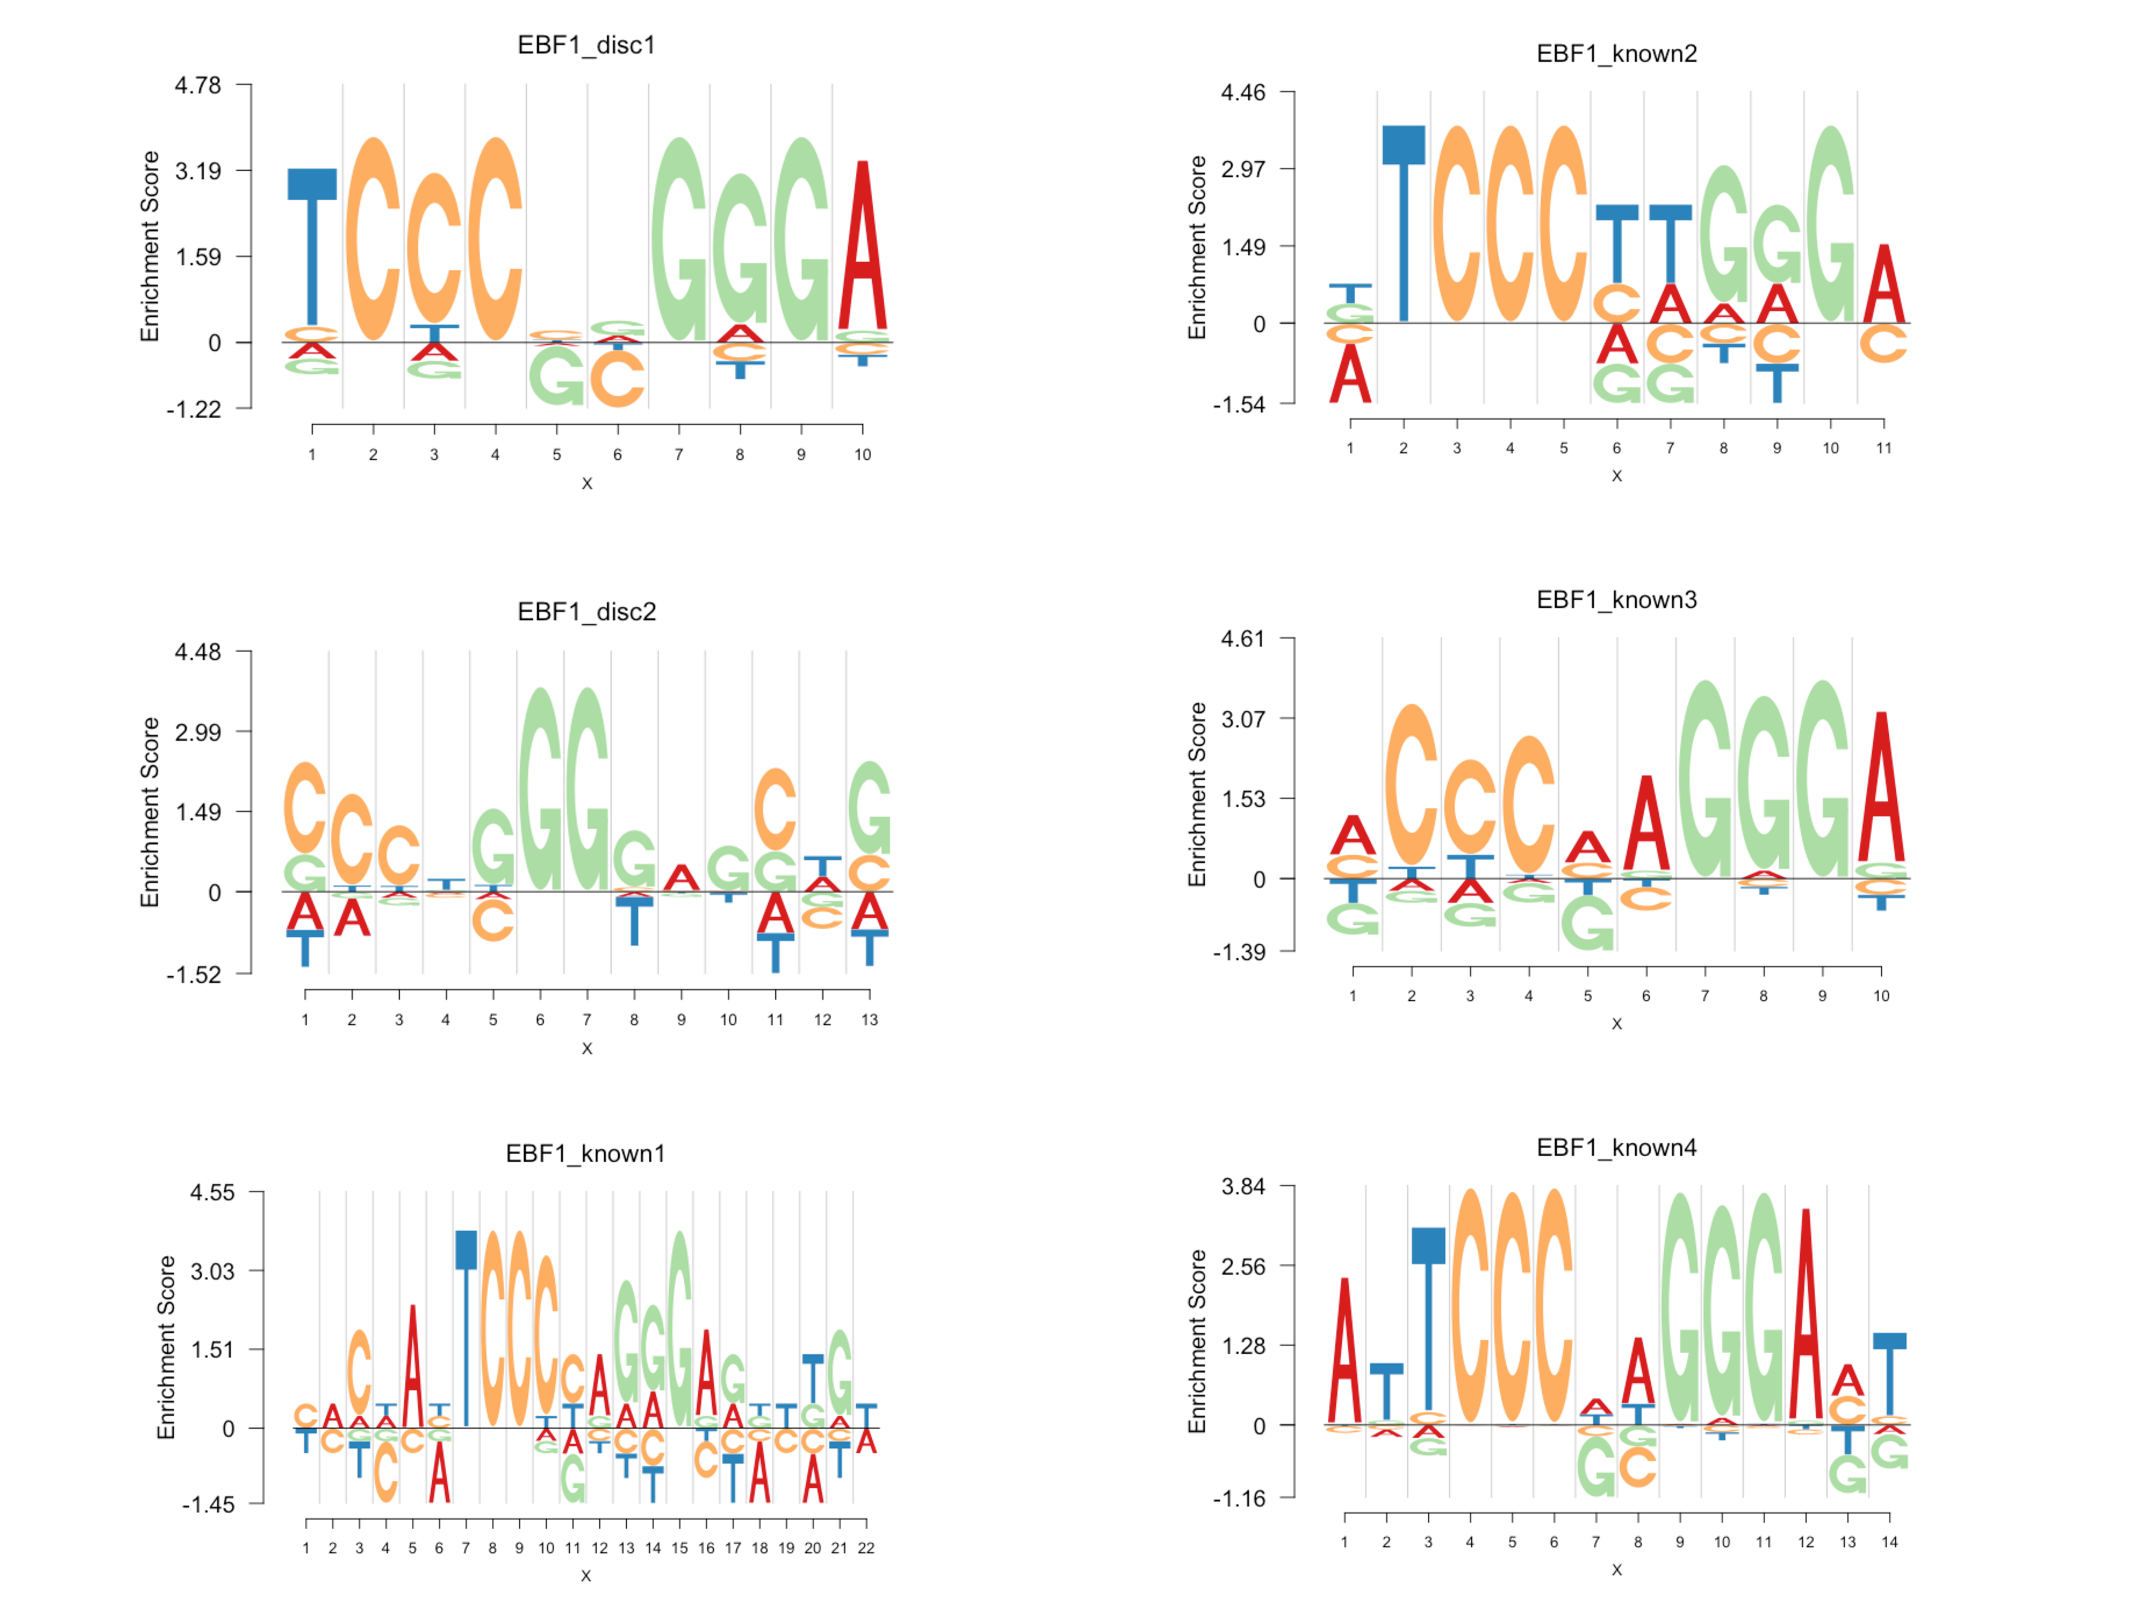
\includegraphics[height=6in, width=7in]{figures_folder/figures6.pdf}
\caption{\textbf{Various approaches of sparse logo representations for a transcription factor} : The sparse logo representation under various stack height and stack composition methods - \textit{log}, \textit{log-odds}, \textit{ratio}, \textit{ic-log}, \textit{ic-log-odds} and \textit{ic-ratio} for the Early B cell factor 1 disc 1 (EBF1-disc1) transcription factor. The data is fetched from the CompBio website of MIT \url{http://compbio.mit.edu/encode-motifs/}}
\label{fig:suppfig4}
\end{figure*}

\begin{figure*}[h!]
\centering
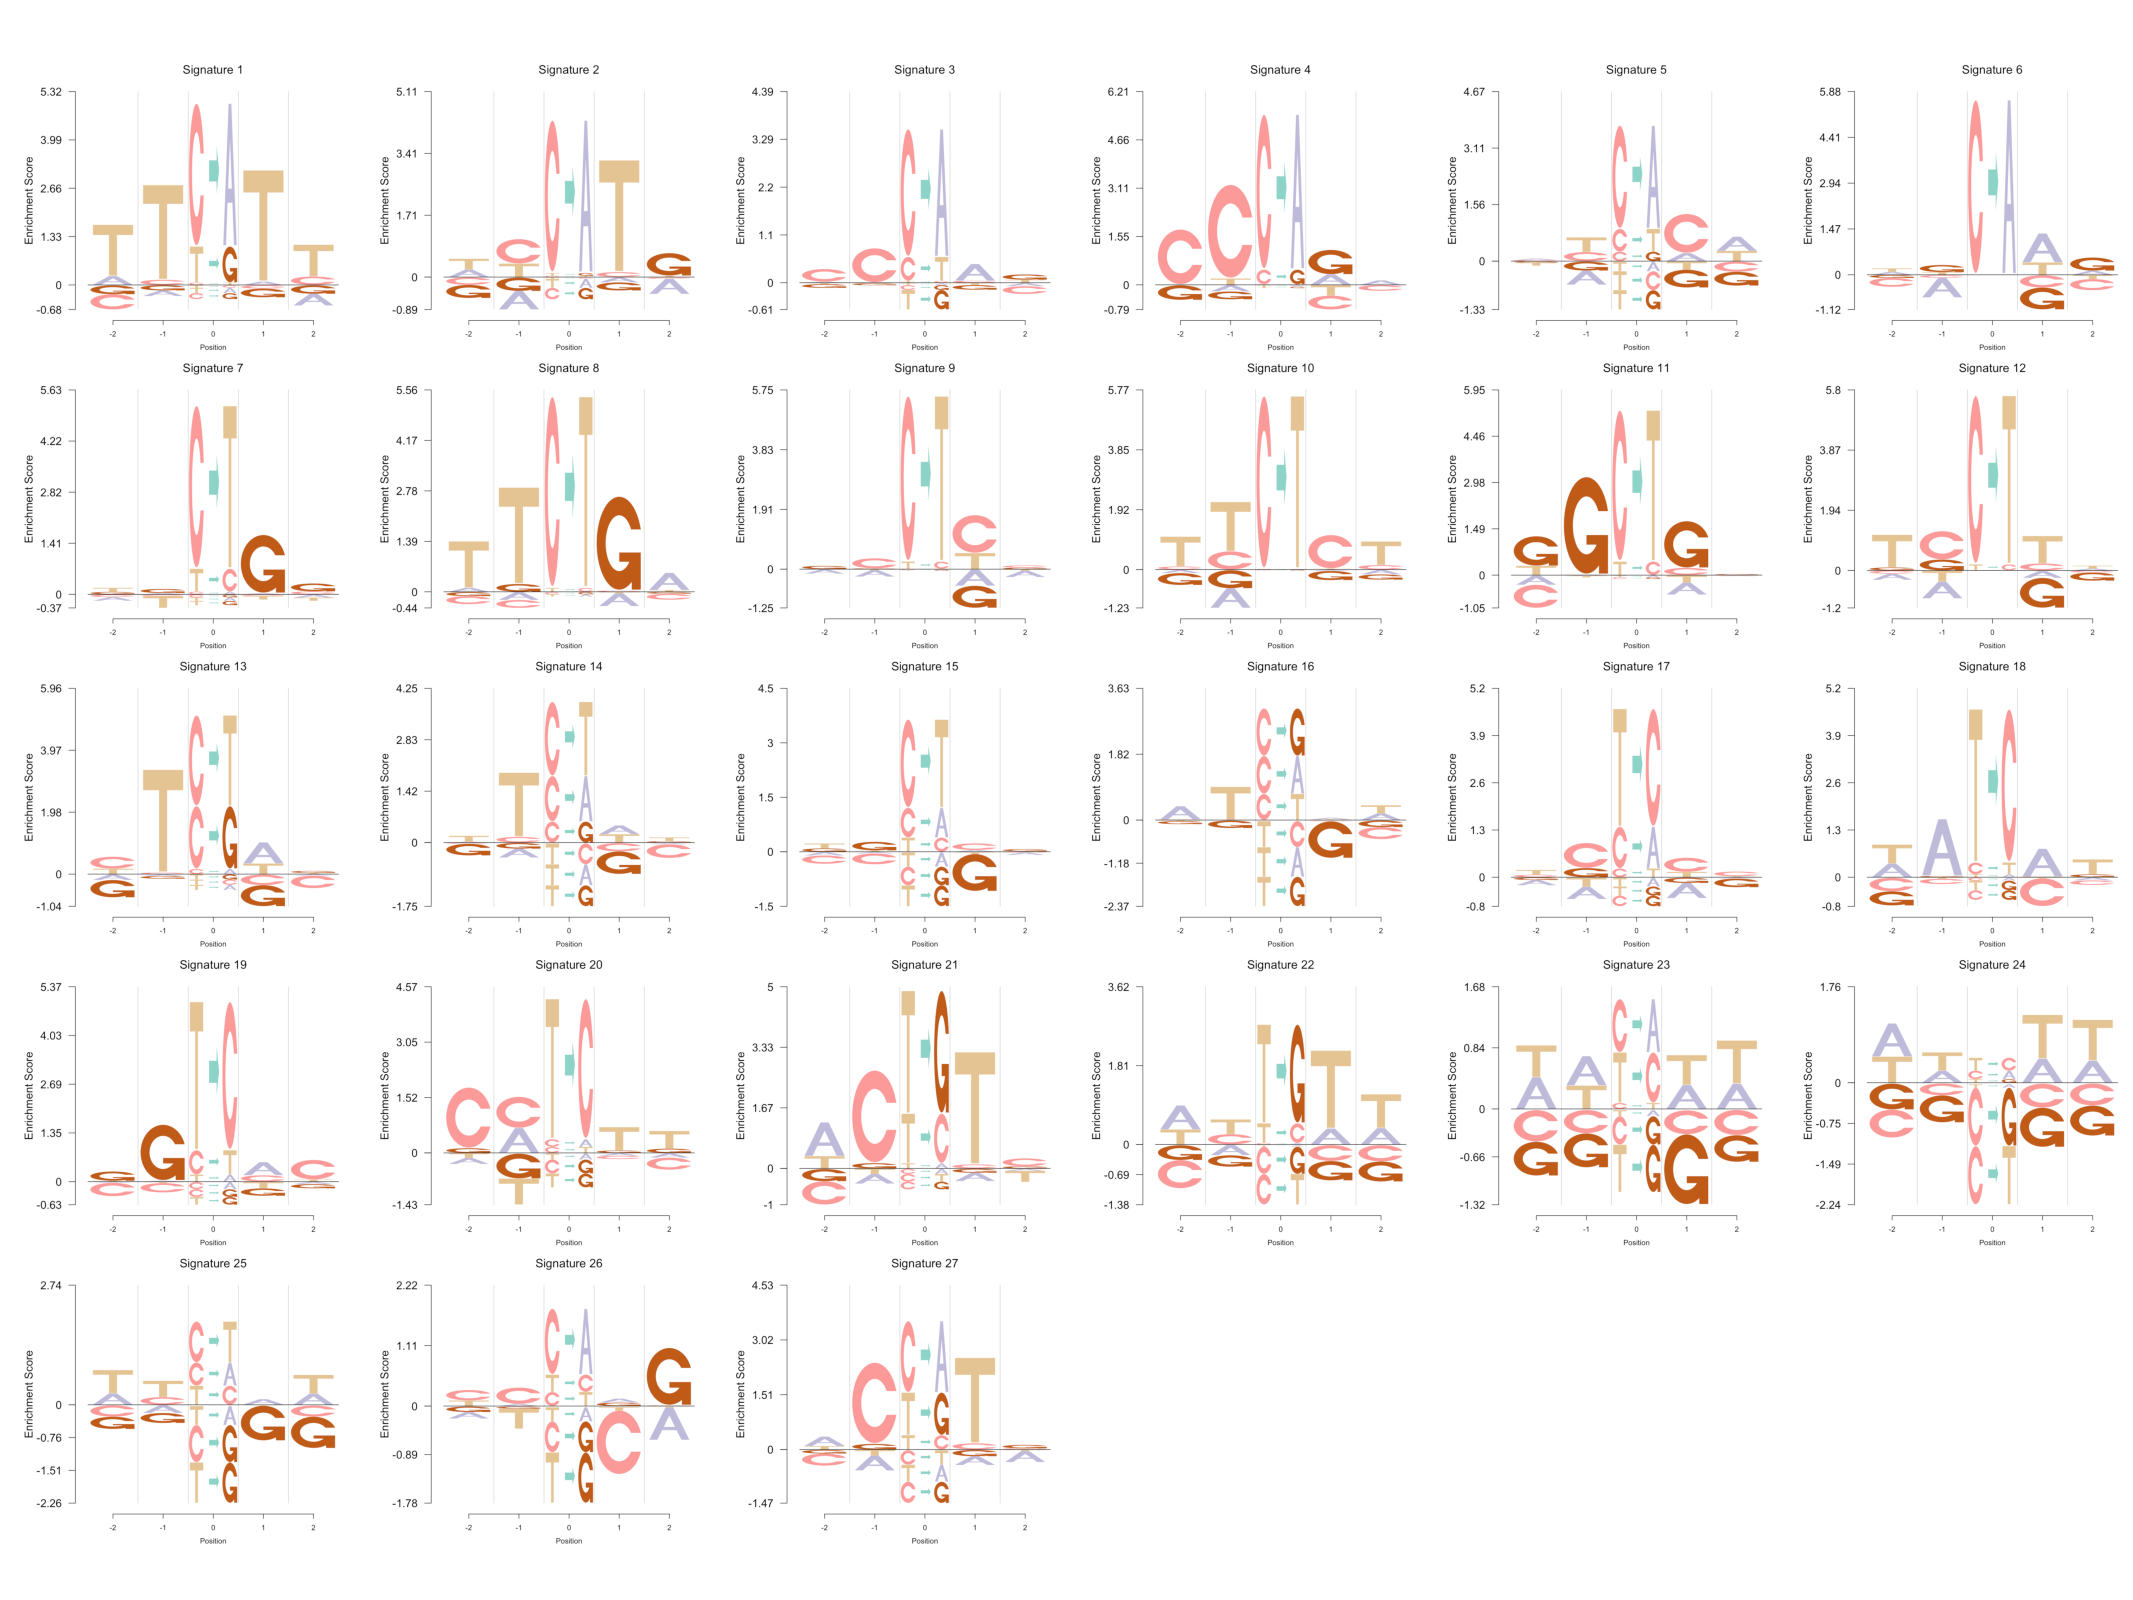
\includegraphics[height=6in, width=7in]{figures_folder/figures11.pdf}
\caption{\textbf{Logolas plots for the mutational signature profiles for 27 clusters in Shiraishi et al (2015)}: 
We present the sparse logo representations (ratio) method for the 27 cluster signature profiles obtained from fitting a grade of membership model on the cancer mutational signature data across 30 cancer types by Shiraishi et al (2015) \cite{Shiraishi2015}. This plot is an alternative logo plot based representation of Figure 4 in Shiraishi et al (2015) \cite{Shiraishi2015}}
\label{fig:suppfig5}
\end{figure*}

\begin{figure*}[h!]
\centering
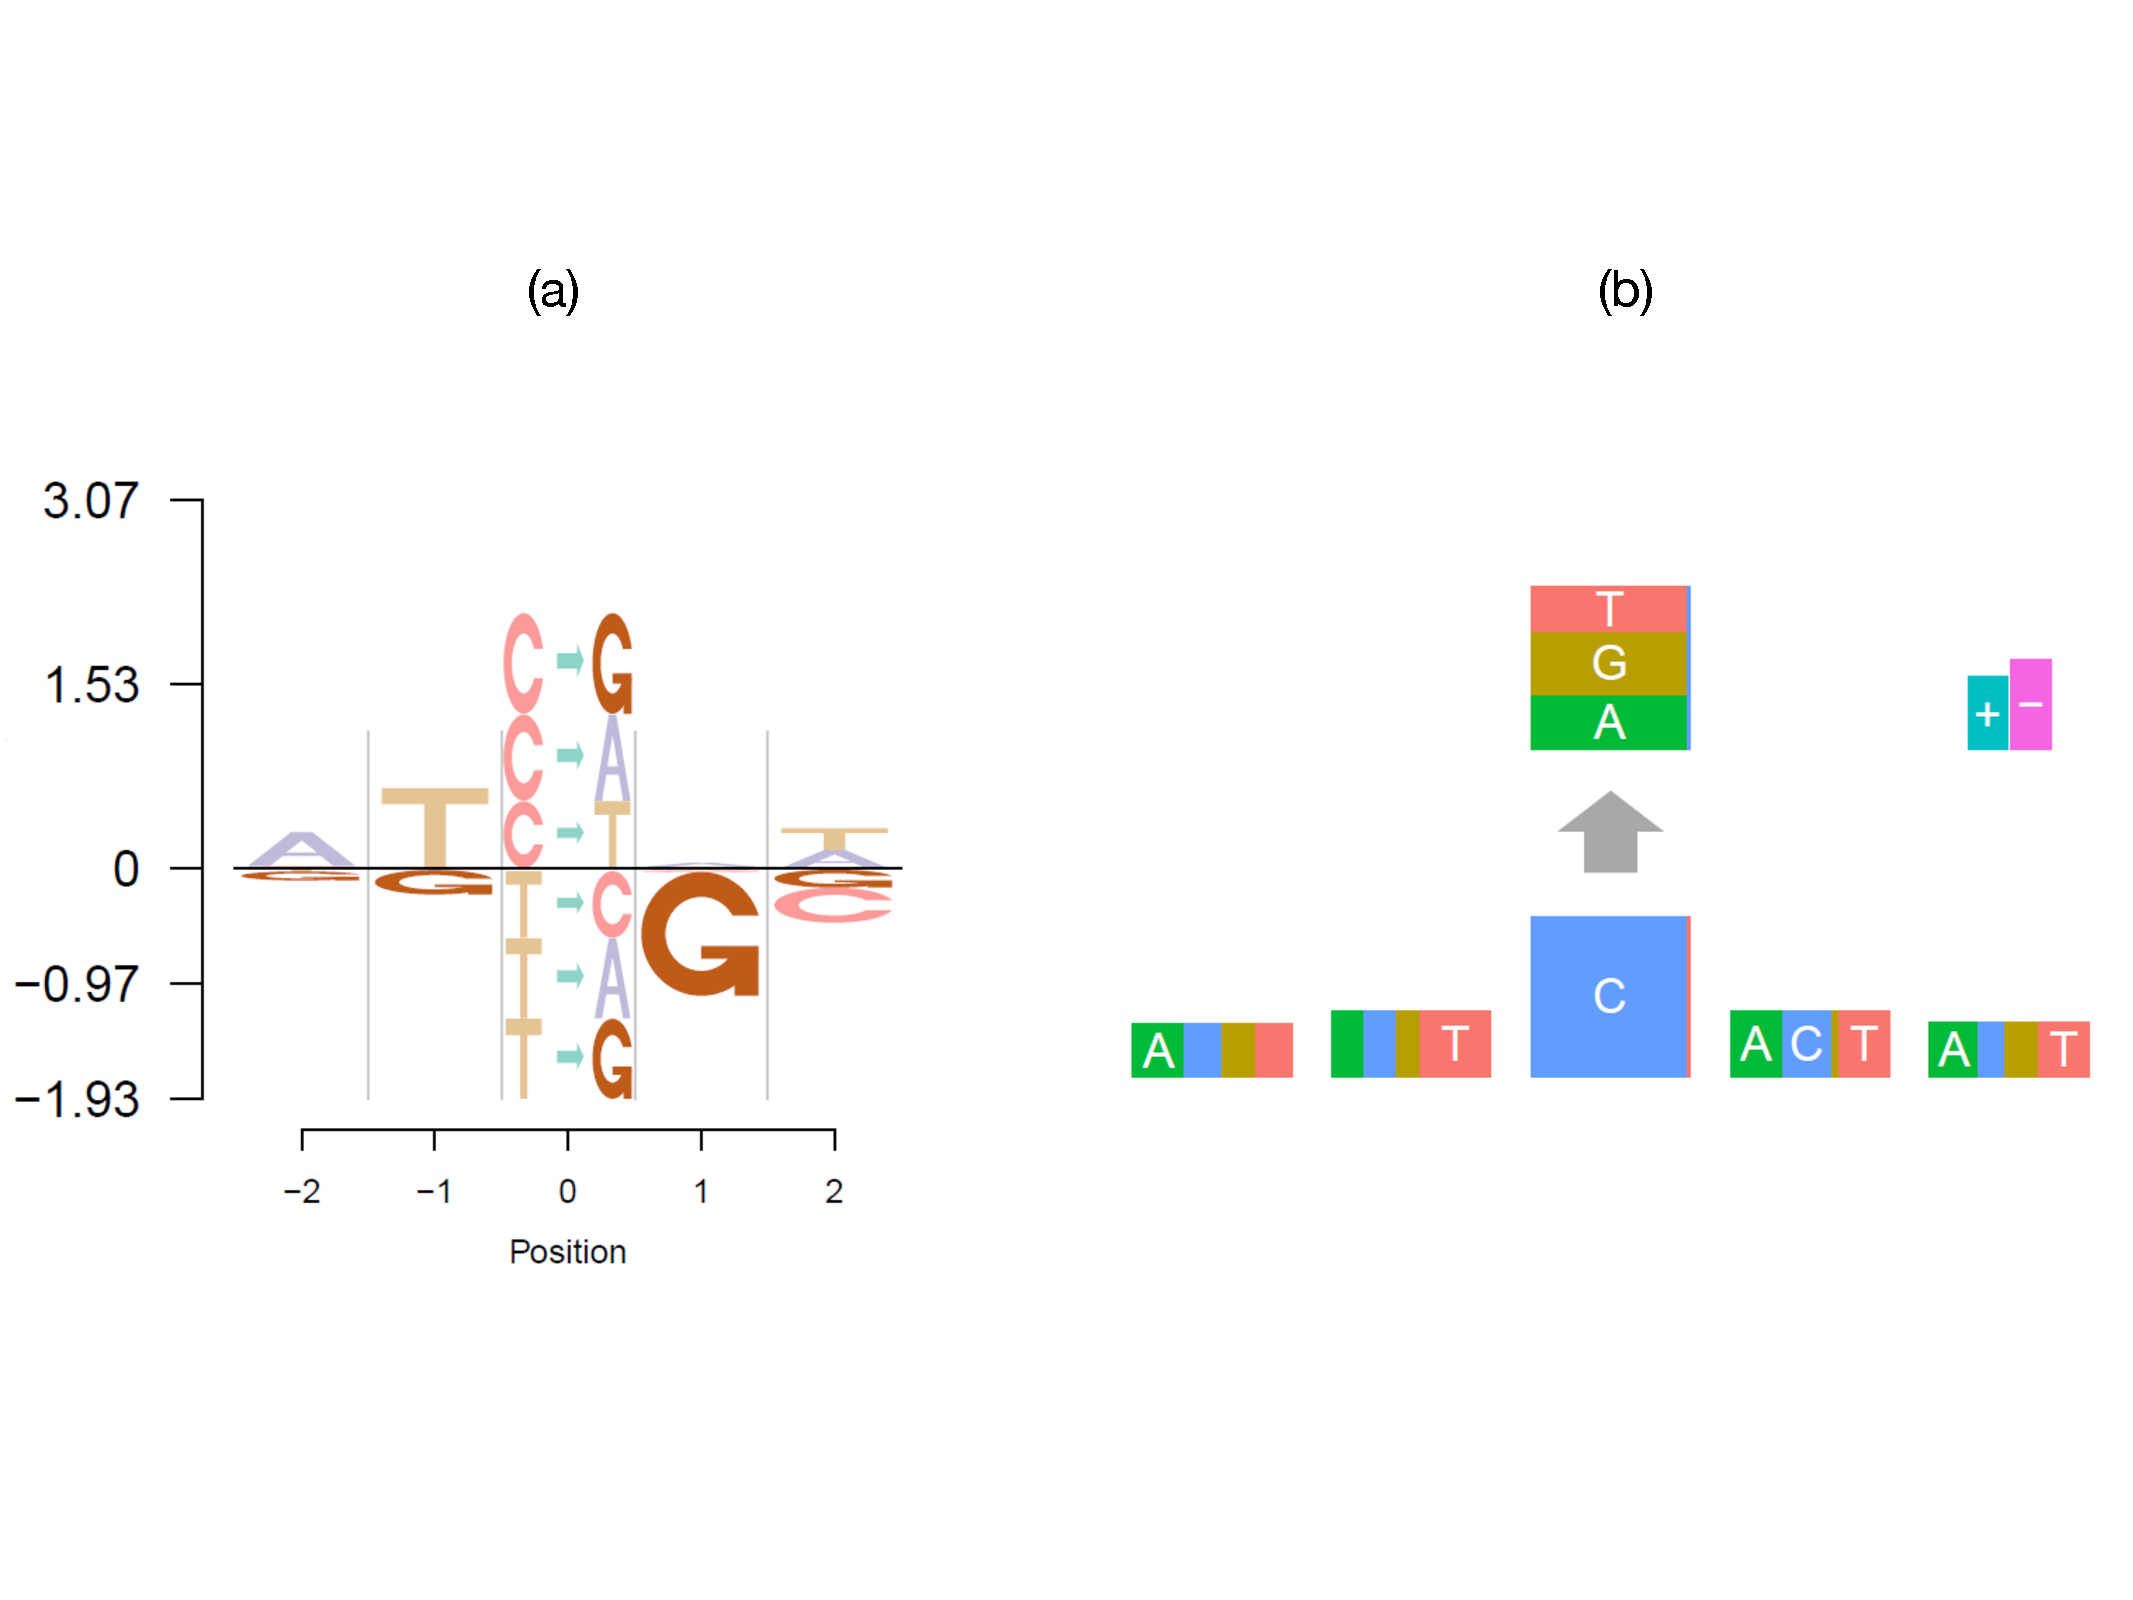
\includegraphics[height=6in, width=7in]{figures_folder/figures2.pdf}
\caption{\textbf{Comparison of Logolas sparse logo plot with pmsignature representation for cancer mutation signatures}: 
We compare the sparse logo plot representation and the pmsignature representation due to Shiraishi et al (2015) \cite{Shiraishi2015} for mutation signature profile of cluster 16 in their paper. The position 0 corresponds to the mutation. Positions $-1$ and $-2$ correspond to the the two left flanking bases with respect to the mutation. Positions $1$ and $2$ correspond to the the two right flanking bases with respect to the mutation. Clearly, the logo plot representation shows the depletion of G at the right flanking base more clearly than the pmsignature plot. Also, overall, the logo plot representation is more interpretable and visually appealing in highlighting the mutation signature patterns compared to the pmsignature plot.}
\label{fig:suppfig6}
\end{figure*}

\begin{figure*}[h!]
\centering
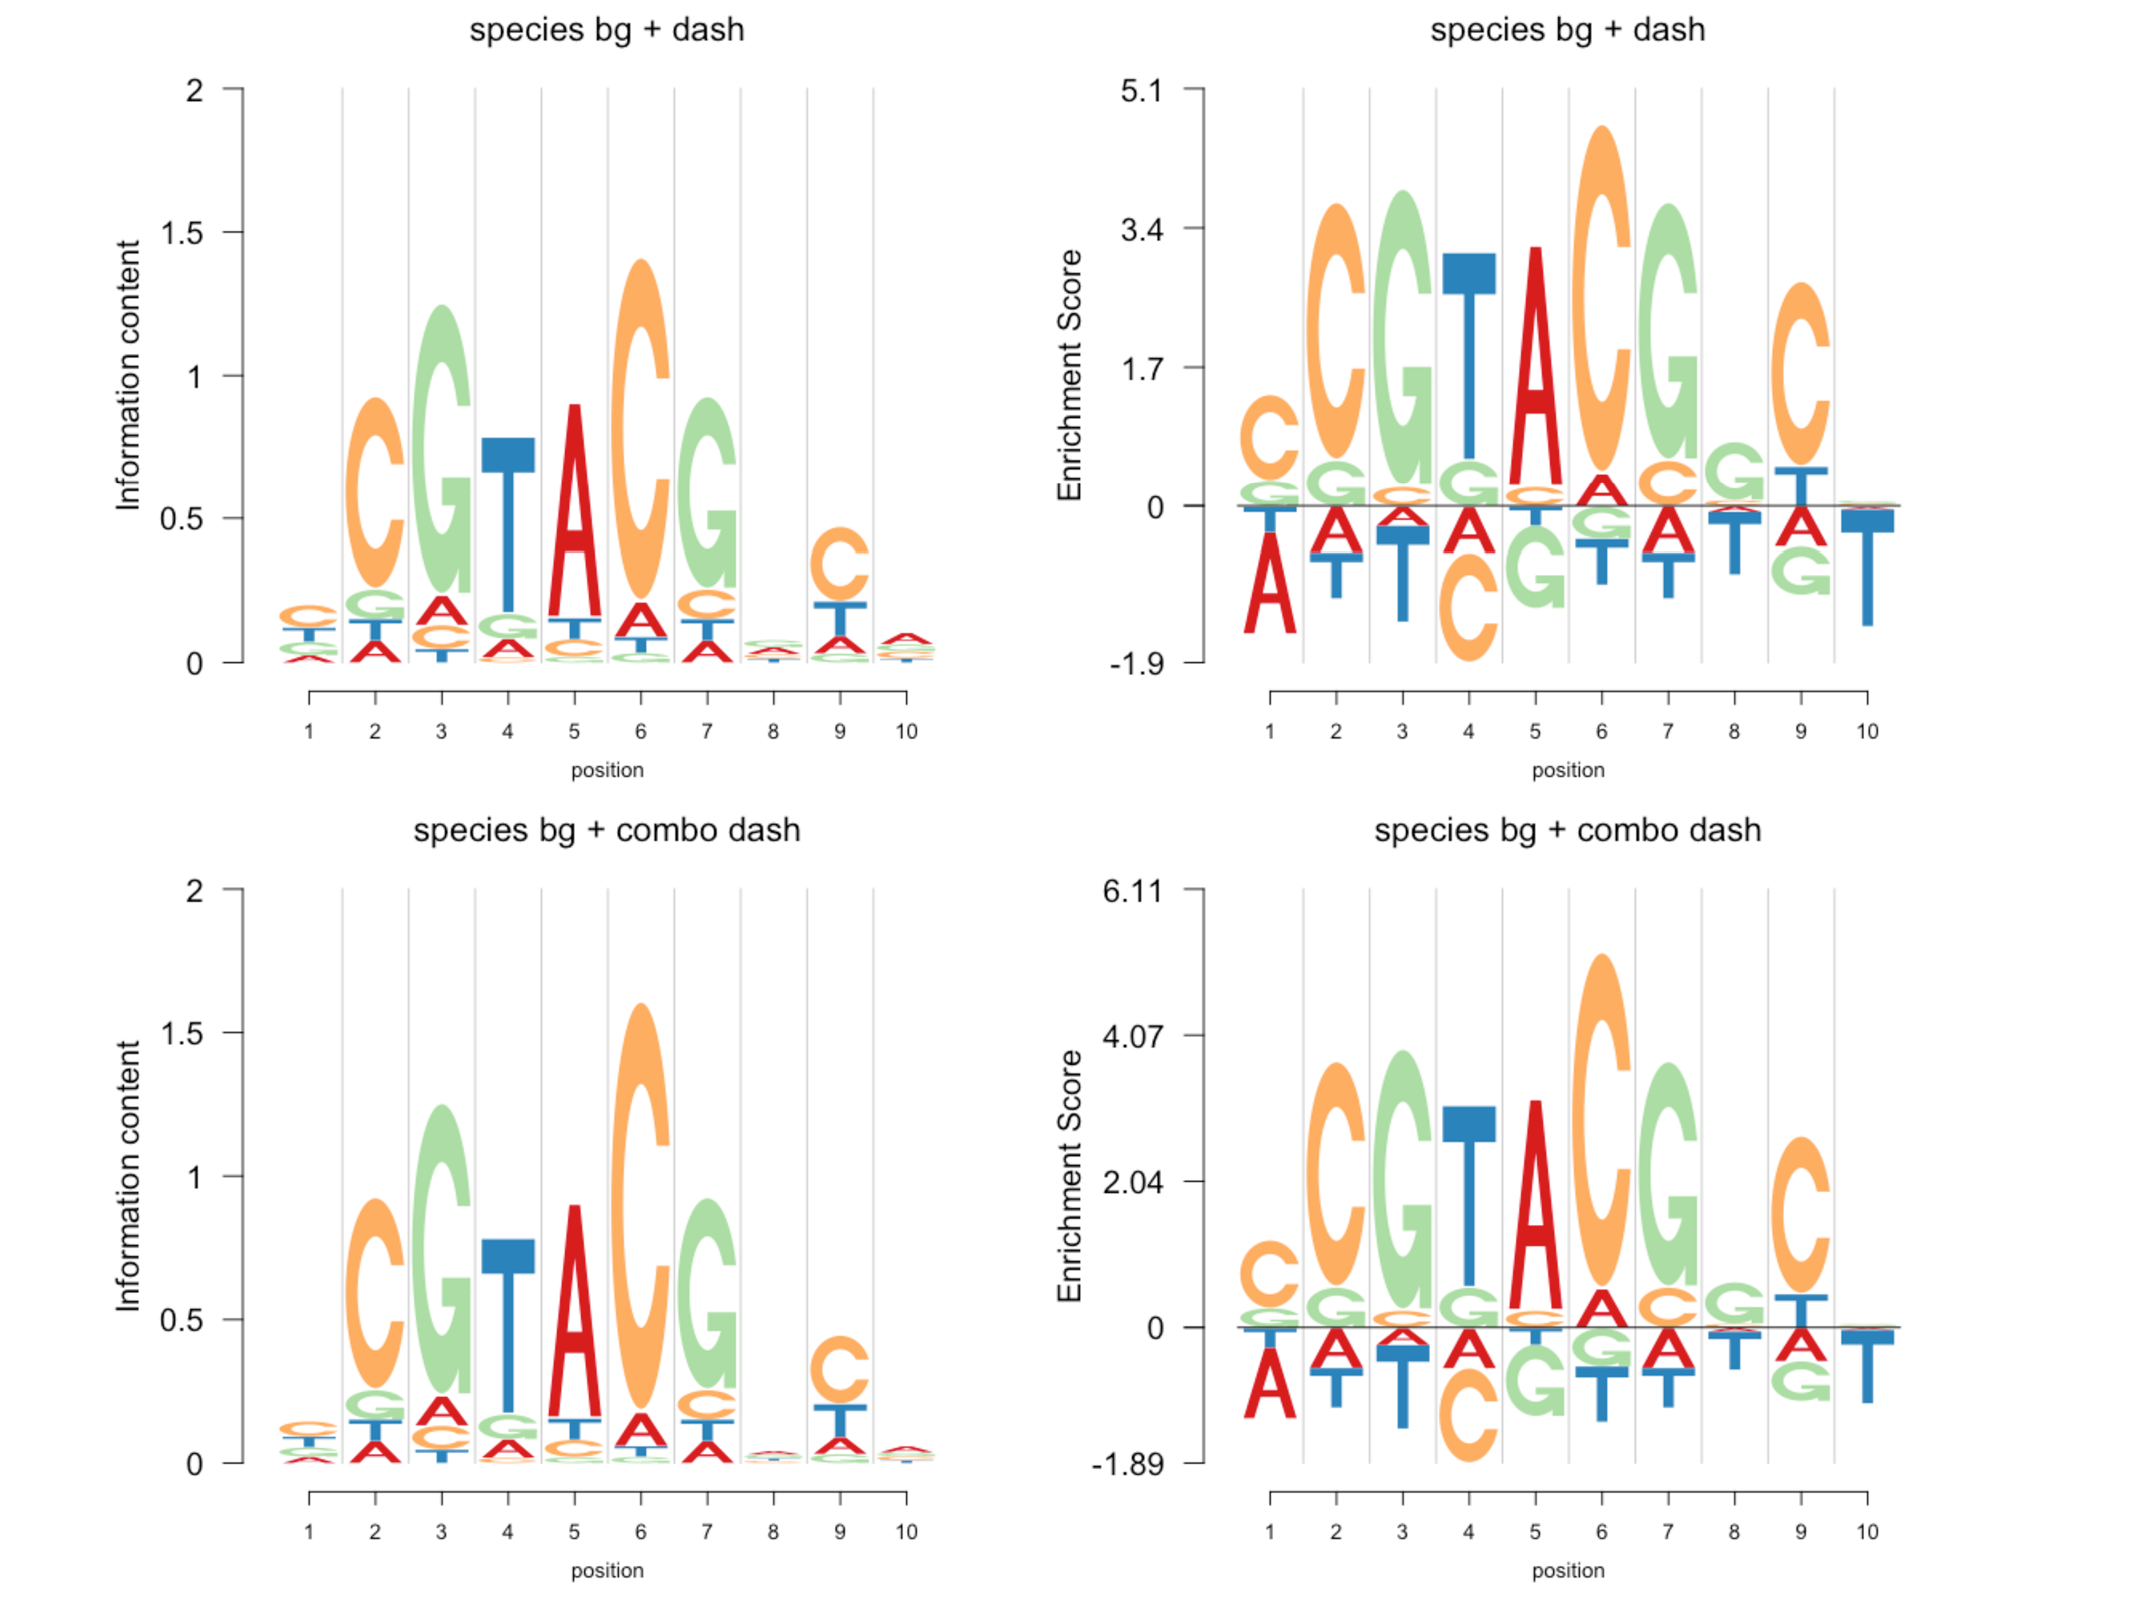
\includegraphics[height=6in, width=7in]{figures_folder/figures15.pdf}
\caption{\textbf{Dirichlet Adaptive Shrinkage (dash) training on combined transcription factor data for a species}: 
We compare the two versions of Dirichlet Adaptive Shrinkage (dash) applied to the SBP protein transcription factor Achn185791 in \textit{Actinidia chinensis}. In one case, the parameters of the \textit{dash} model are learnt from the positional frequency data from Achn185791, while in the other case, the the parameters are learnt from the pooled positional frequency data across all 290 transcription factors of \textit{Actinidia chinensis}, which we refer to as \textit{combo dash} in this plot. The background probability of the bases for this species are $ q = \left( q_A, q_C, q_G, q_T \right ) = \left (0.3141, 0.1859, 0.1859, 0.3141 \right ) $. The transcription factor data for 
\textit{Actinidia chinensis} along with the background probability information are derived from the PlantTFDB v4.0 database \url{http://planttfdb.cbi.pku.edu.cn/index.php?sp=Ach}. }
\label{fig:suppfig7}
\end{figure*}

\begin{figure*}[h!]
\centering
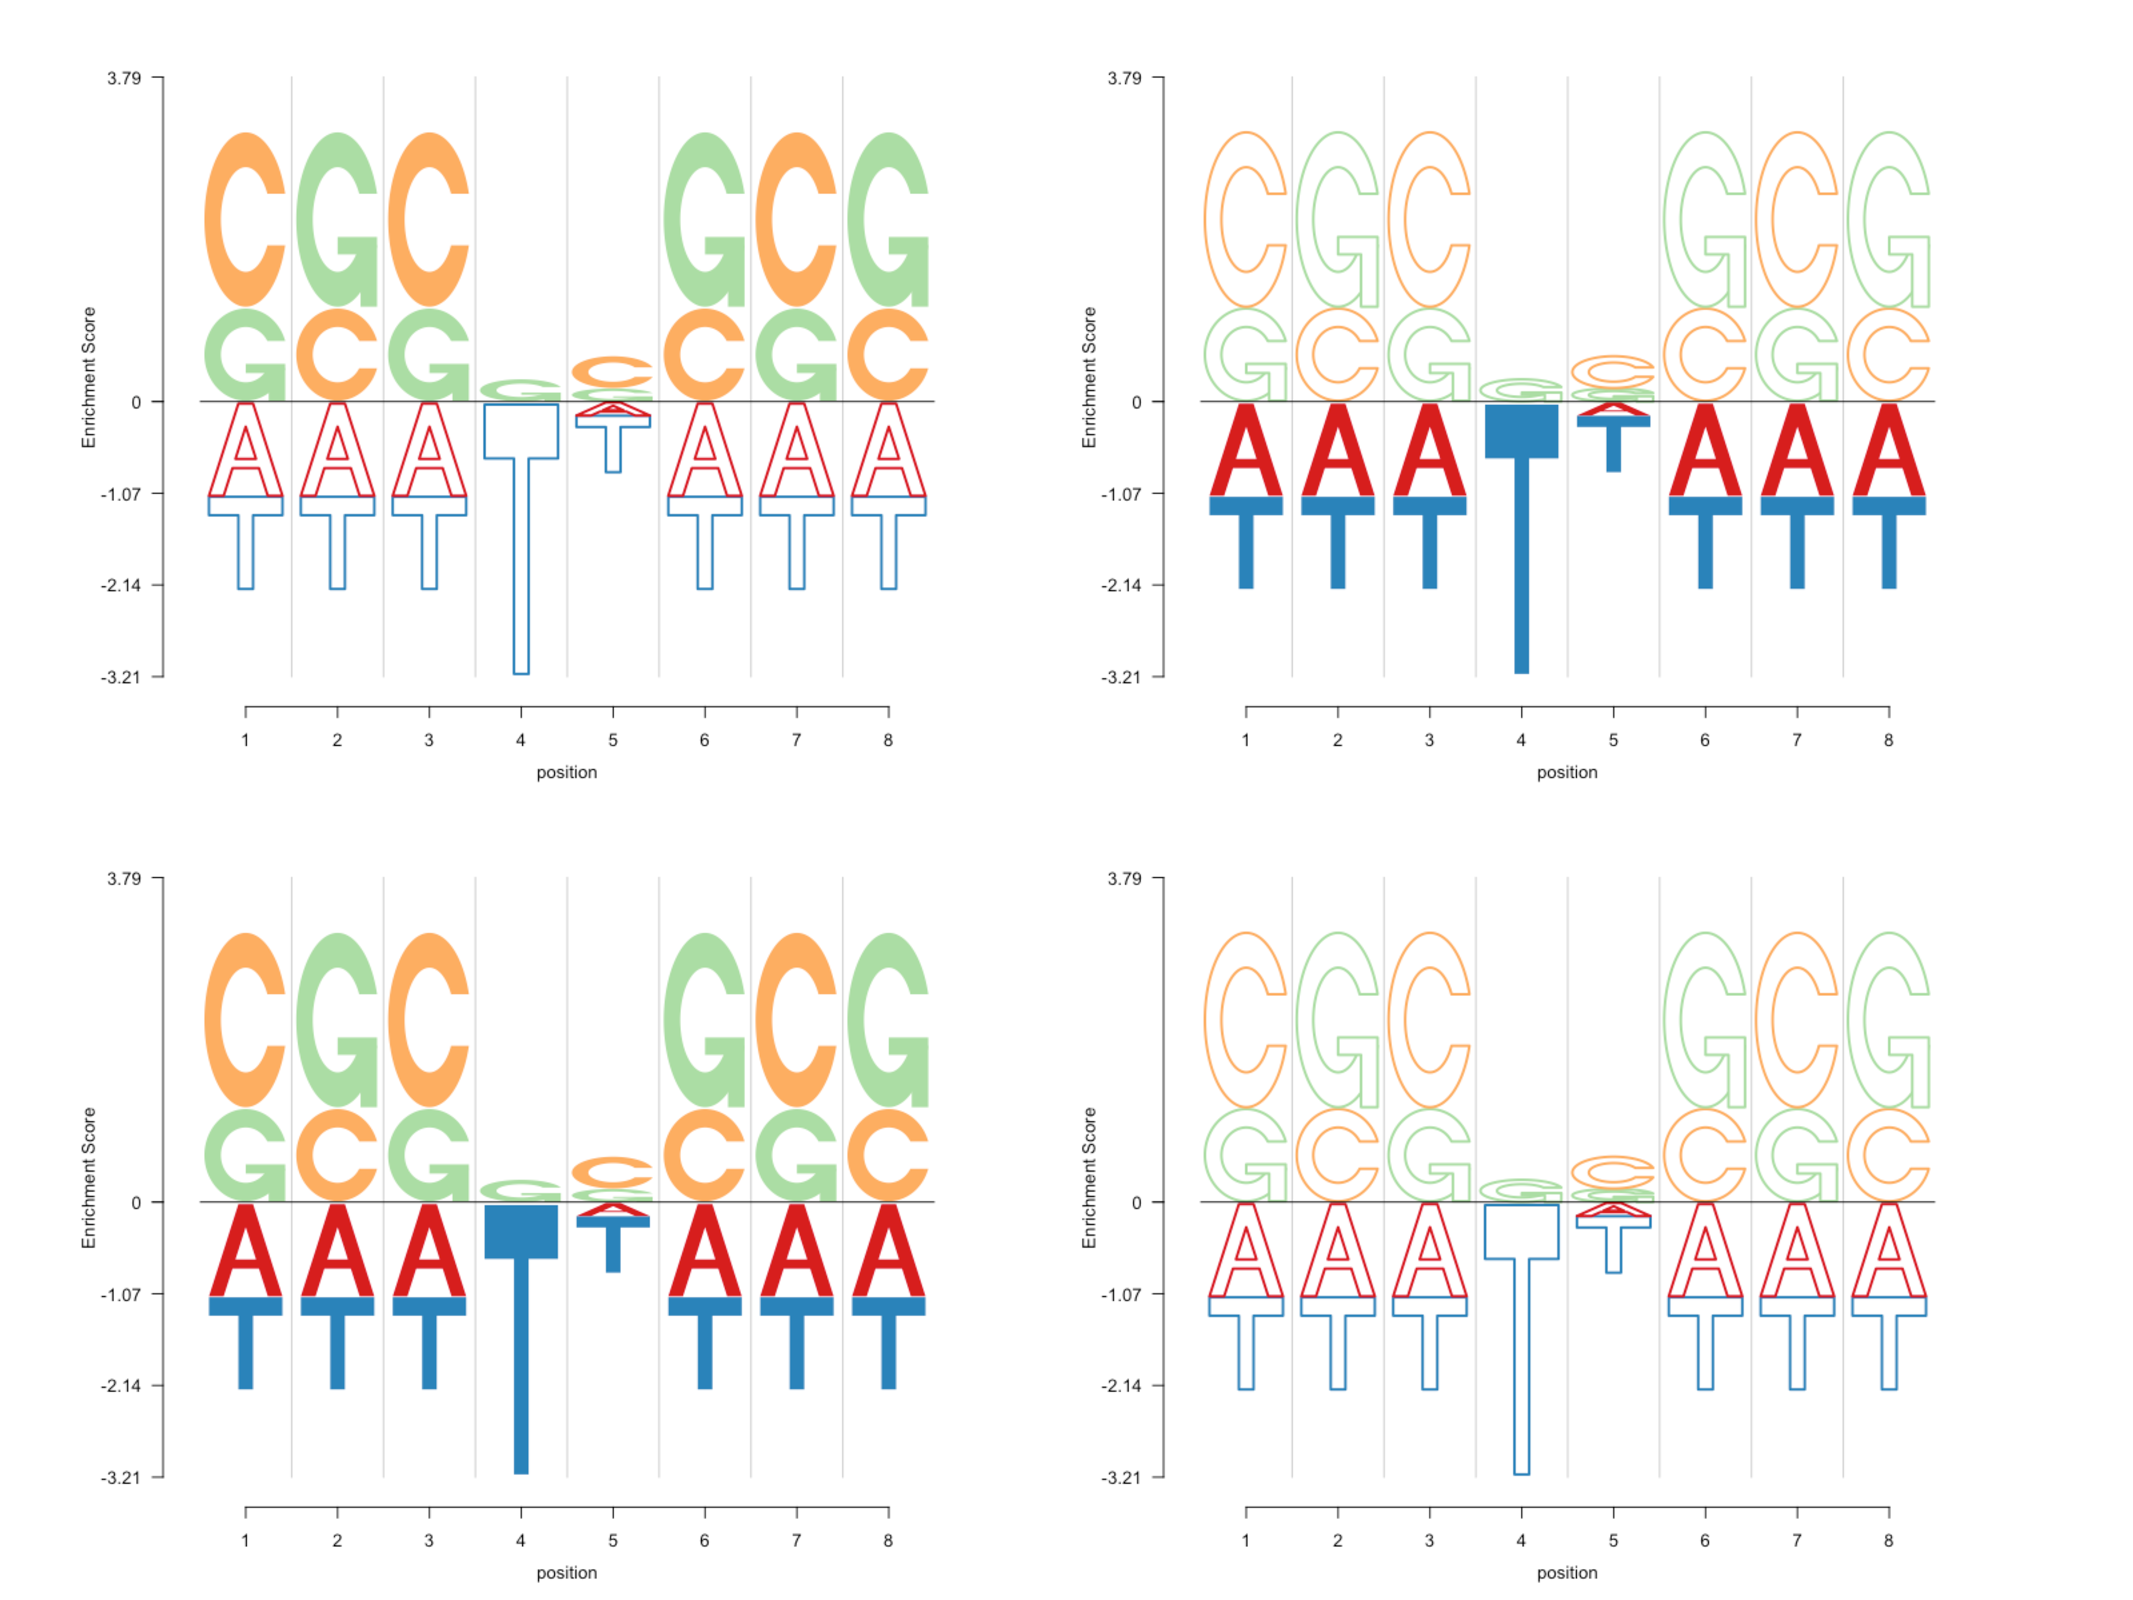
\includegraphics[height=6in, width=7in]{figures_folder/figures9.pdf}
\caption{\textbf{Fill and border styles in Logolas.}:
A demonstration of how fill and border styles can be used to distinguish between the enrichment and depletion of symbols at a position in a sparse logo plot.}
\label{fig:suppfig8}
\end{figure*}

\begin{figure*}[h!]
\centering
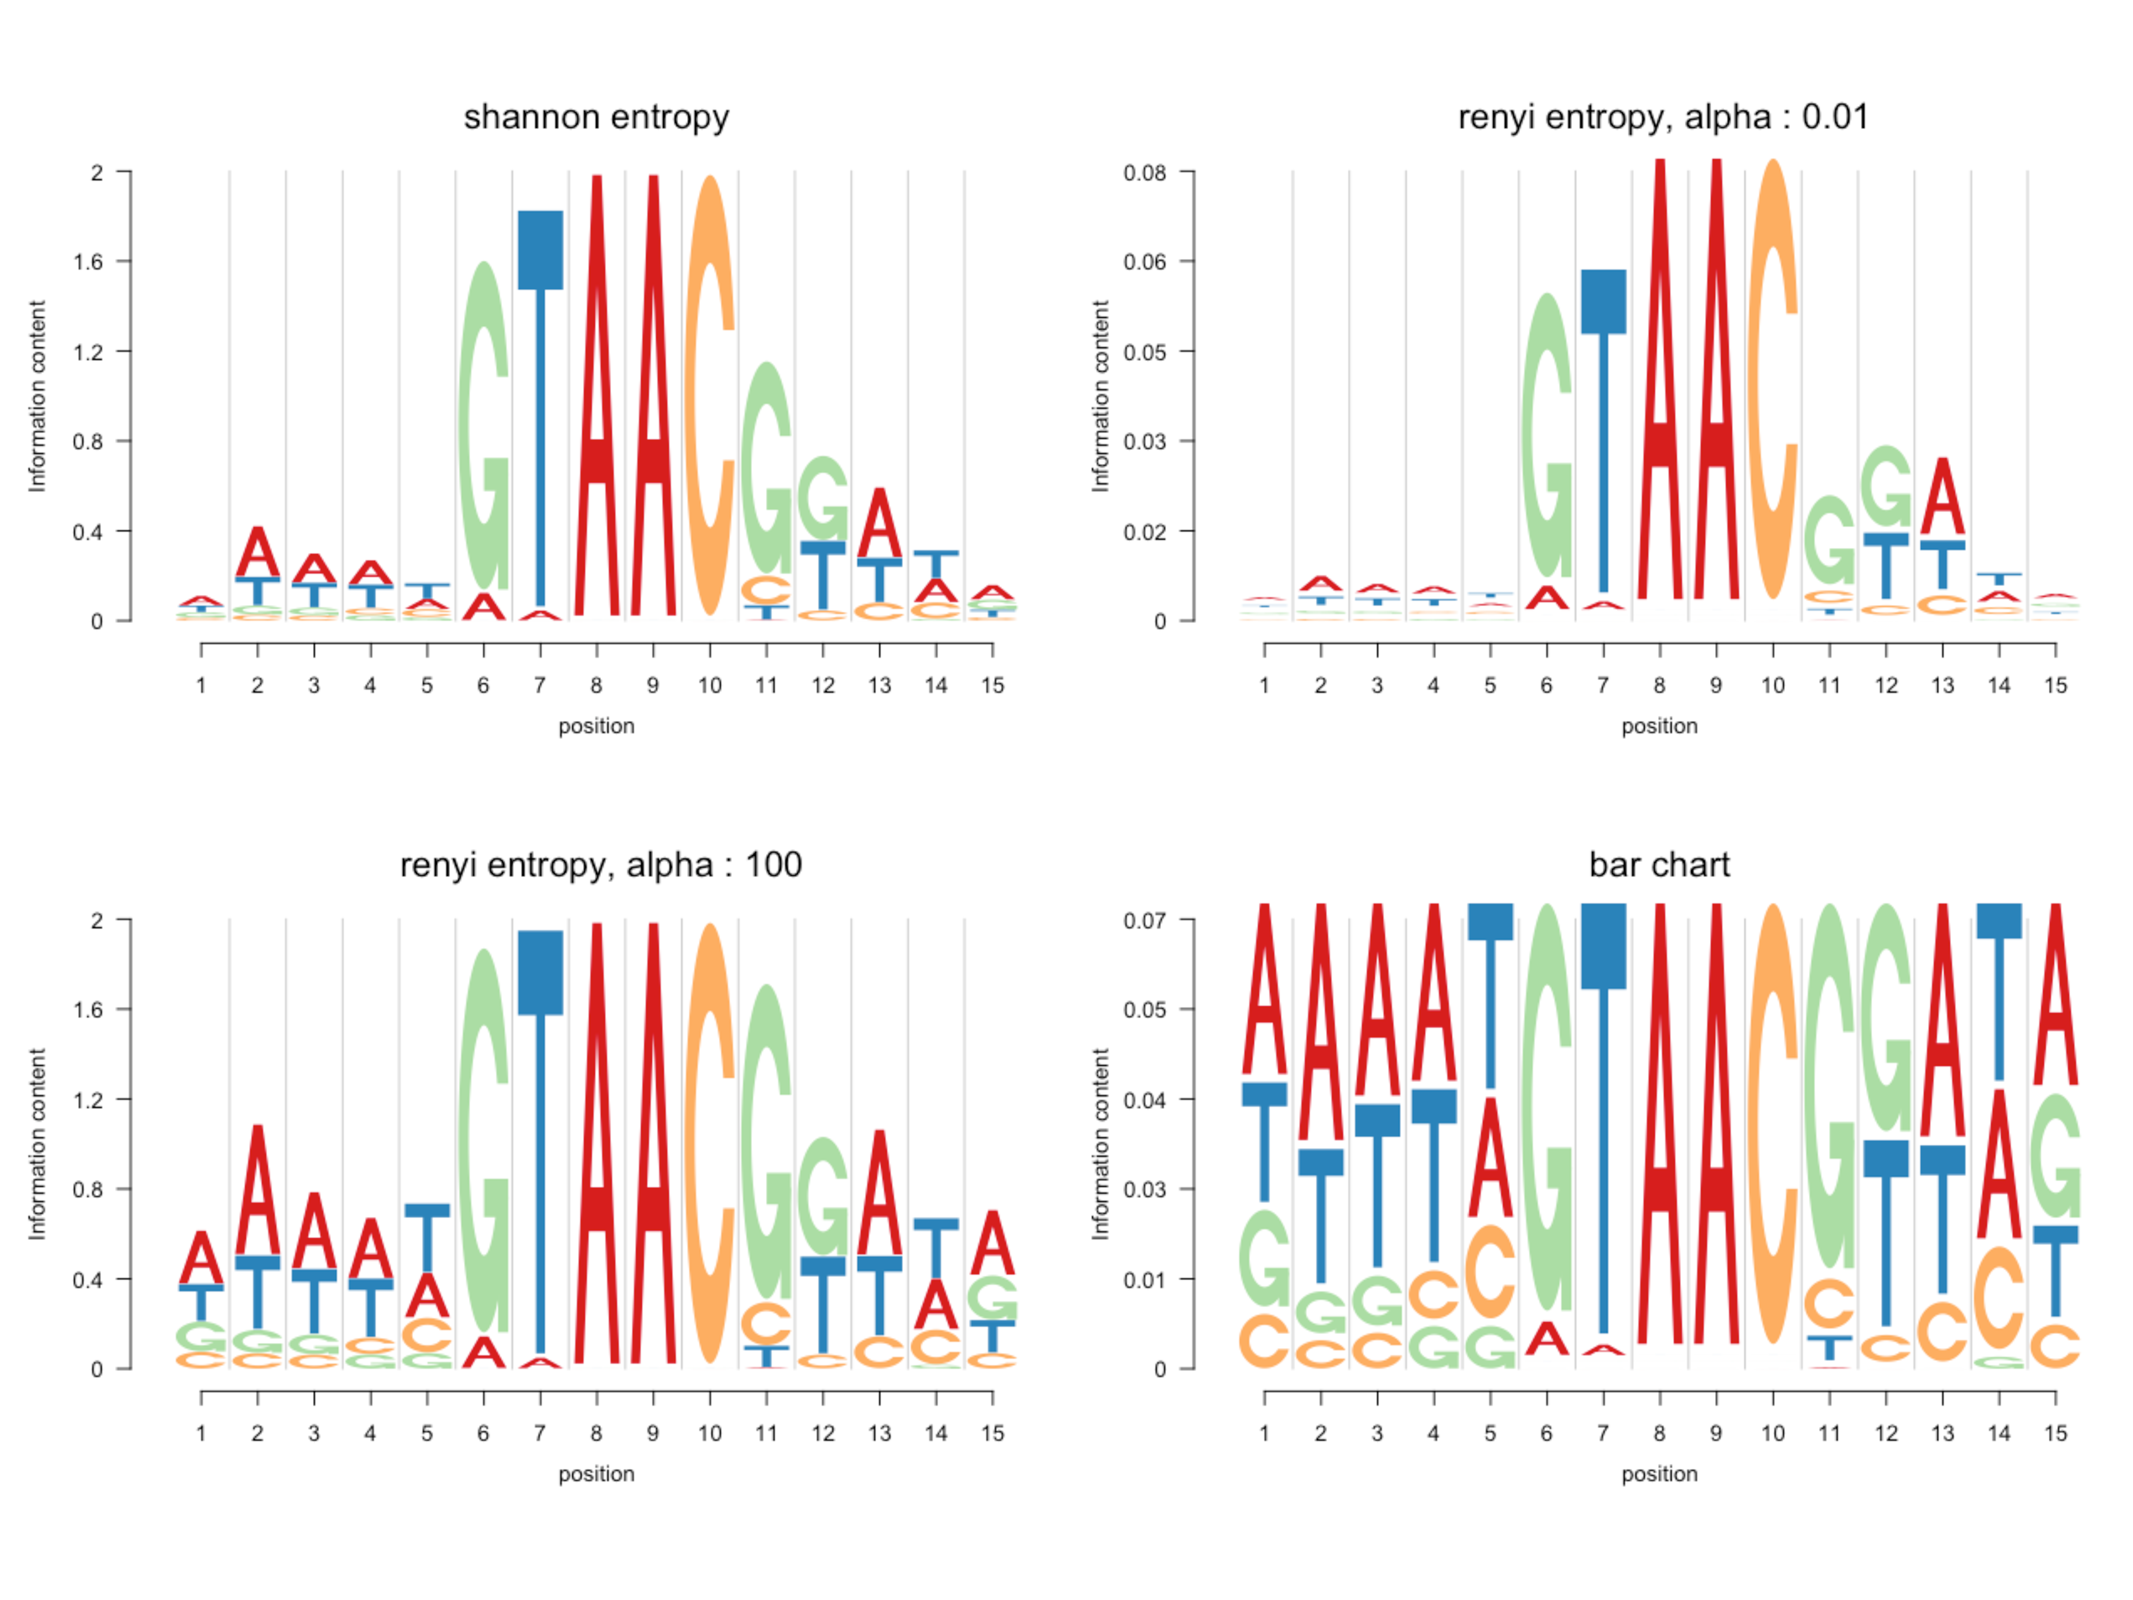
\includegraphics[height=6in, width=7in]{figures_folder/figures12.pdf}
\caption{ \textbf{Stack heights in Logolas.} : 
 A demonstration of how stack height for a position in a standard logo plot can be determined in various ways in \textit{Logolas}. In panel (a), the standard Shannon entropy based Information content is used to determine the height of the stack of symbols at each position. For panels (b) and (c), we use Renyi entropy based information content for two levels of tuning parameter $\alpha$, one when $\alpha = 0.1$ is small and the other when $\alpha =100$ is large. In panel (d), a relative frequency based stacked bar chart representation using logos is implemented. All these options can be passed as input arguments and control arguments to the \textit{logomaker} functon in \textit{Logolas}.}
\label{fig:suppfig8}
\end{figure*}

\end{document}
